%% Template for EU deliverable, using the deliverable.sty style file

\documentclass[12pt,a4paper,twoside]{article}

%% common package
\usepackage[headers]{deliverable}
\usepackage{xspace}
\usepackage{verbatim}
\usepackage[usenames]{color}
\usepackage[usenames,dvipsnames]{xcolor}
\usepackage{graphicx}
\usepackage{url}
\usepackage{array}
\usepackage{amsmath,bm,amsfonts}
\usepackage{tikz}
\usetikzlibrary{arrows,automata}
\usepackage{IEEEtrantools}
\usepackage{mathtools}
\DeclareMathOperator*{\argmin}{argmin}


\usepackage{times}

% numbers option provides compact numerical references in the text. 
\usepackage[numbers]{natbib}
\usepackage{multicol}
\usepackage[bookmarks=true]{hyperref}

\usepackage{graphicx,import}
\usepackage{mathtools, amssymb}
\usepackage{paralist}
\usepackage[pdf]{svg}
\usepackage{amsmath,amssymb,amsthm}

% \pdfinfo{
%    /Author (Homer Simpson)
%    /Title  (Robots: Our new overlords)
%    /CreationDate (D:20160128120000)
%    /Subject ()
%    /Keywords (Robotics;)
% }

\newtheorem{assumption}{\bf{Assumption}}
\newtheorem{definition}{\bf{Definition}}
\newtheorem{boldLemma}{\bf{Lemma}}
%%

%%insert here other packages needed by sections

%%

%%%%%%%%%%%%%%%%%%%%%%%%%%%%%%%%%%%%%%%%%%%%%%%%%%%%%%%%%%%%%%%%%%%%%%%%%%%%%%
%%% Titlepage
%%%%%%%%%%%%%%%%%%%%%%%%%%%%%%%%%%%%%%%%%%%%%%%%%%%%%%%%%%%%%%%%%%%%%%%%%%%%%%

% declaration of variables used in style
\deliverableDocnumber{D5.3}
\deliverableTitle{Validation scenario 3: \\ balancing on compliant environmental contacts}

\deliverableAuthor{Daniele Pucci}
\deliverableResponsiblePartner{IIT}
\deliverableAffiliation{% Insert here authors affiliations
 $^1$ IIT
}

\deliverableReviewer{Daniele Pucci}
\deliverableCoordinator{Daniele Pucci}
\deliverableActivityNumber{n} %% n=1,..,10
\deliverableActivity{RTD}
\deliverableDoctype{Deliverable} %% or Prototype
\deliverableClassification{Public} % or Consortium
\deliverableDistribution{Consortium} %
\deliverableStatus{Draft} % Draft or Final
\deliverableDeliveryDate{28/2/2016}
\deliverableFile{D5.2.pdf} % please do not use "-" in the name
\deliverableVersion{1.0}
\deliverableDate{Feb.~28, 2016}
\deliverableYear{2015}
\deliverablePages{\pageref{LastPage}}
\deliverableChangelog{v.1.0 & Feb 19, 2015 & First draft %%\\\hline
%%              v.2.0 & Feb 20, 2007 & Final version
}
\deliverableProjectStartingDate{1st March 2013}
\deliverableProjectEndDate{28th February 2017}
\deliverableProjectAcronym{CoDyCo}
\deliverableProjectTitle{Whole-Body Compliant Dynamical Contacts in Cognitive Humanoids}
 \deliverableContractNumber{600716}
 \deliverableProjectCoordinator{Istituto Italiano di Tecnologia}
 \deliverableProjectUrl{www.codyco.eu}
 \deliverableFrameworkProgramme{FP7}
 
 \deliverableWorkpackage{deliv WP5}
 \deliverableEditors{Daniele Pucci}
 \deliverableContributors{Daniele Pucci, Francesco Romano, Jorhabib Eljaik, Silvio Traversaro, Vincent Padois, Francesco Nori}
 \deliverableReviewers{}
\deliverableAbstract{This deliverable discusses the technical details and choices for the implementation of the year-3 validation scenario of the CoDyCo project.  The validation scenario aims at verifying the control performances in the case the humanoid robot iCub must balance  by means of  compliant or dynamical contacts. With \emph{dynamical contact} we mean that the robot's link in contact with the environment is not fixed with respect to an inertial frame, and the wrench applied to it is not due to a spring-damper system. First, we detail the control algorithm for dealing with a soft carpet underneath the robot's feet. This case study exemplifies the case of a robot interacting with a compliant environment. Then, we present the control algorithm to allow the robot balancing on a semi-cylindrical seesaw. This case study exemplifies the  problem of a humanoid robot  balancing by means of dynamical contacts. In fact, the robot's feet do not have a constant pose with respect to the inertial frame in this case. Contact and trajectory planning are not part of the scenario. }
\deliverableReviewers{}
\deliverableKeywordList{Multiple, compliant, dynamical, contacts, control, stability, tracking, forces, torques.}

%%%%%%%%%%%%%%%%%%%%%%%%%%%%%%%%%%%%%%%%%%%%%%%%%%%%%%%%%%%%%%%%%%%%%%%%%%%%%%
%%% Sections
%%%%%%%%%%%%%%%%%%%%%%%%%%%%%%%%%%%%%%%%%%%%%%%%%%%%%%%%%%%%%%%%%%%%%%%%%%%%%%


%%
%%%%%%%%%%%%%%%%%%%%%%%%%%%%%% BEGIN DOCUMENT
\begin{document}

\deliverableMaketitle

%%TODO move to style
\newcolumntype{L}[1]{>{\raggedright\let\newline\\\arraybackslash\hspace{0pt}}m{#1}}
\newcolumntype{C}[1]{>{\centering\let\newline\\\arraybackslash\hspace{0pt}}m{#1}}
\newcolumntype{R}[1]{>{\raggedleft\let\newline\\\arraybackslash\hspace{0pt}}m{#1}}

\textbf{Document Revision History}
\begin{center}
\begin{tabular}{|C{2cm}|C{3cm}|p{5cm}|C{4cm}|}
\hline
\textbf{Version}&\textbf{Date}&\textbf{Description}&\textbf{Author}\\\hline
First draft & 19 Feb 2016 & In this version we simply write down a few considerations on the third year validation scenario as discussed after the mid-year CoDyCo meeting in Birmingham. & Daniele Pucci \\\hline
\end{tabular}
\end{center}
 
 \clearpage

\newpage
\renewcommand*\contentsname{Table of Contents}
\renewcommand*\listfigurename{Index of Figures}
\tableofcontents
\newpage
\newpage

%%%%%%%%%%%%%%%%%%%%%%%% Start deliverable content here.

\section{Introduction}

Differently from  the first and second year validation scenarios, the third year CoDyCo  scenario  consists in adding compliance and dynamicity of the robot contacts while the humanoid attempts at balancing.  This kind of situations have not received much attention from the control community,  and the  solutions presented in this document are original in several aspects. 

As in the previous validation scenarios, the control objective is  the regulation of the robot momentum. The rate-of-change of this momentum  equals the summation of all external wrenches applied to the system, and controlling the external wrenches to stabilize the robot's momentum is a known control strategy for humanoids when balancing. One of the main difficulties when dealing with compliant and dynamical contacts in this context comes from the fact that the external wrenches may not be  instantaneously related to the robot's torques, i.e. the input to the system. 
This is the case, for instance, of a humanoid standing on two springs, which exert forces on the robot's feet that depend on the relative compressions only. 

There may be some particular soft terrains, however, that exert forces and torques not only depending on the relative compressions, but also on the robot's joint torques. In these cases, the soft terrain is subject to some rigid constraints that may allow the control of the robot's momentum through the external forces, which thus depend on the joint torques. This is the case of a thin, highly damped carpet, which can be modeled, in the first approximation, as a continuum of vertical springs. Each of these springs is assumed to compress vertically only, and the other degrees of freedom are rigidly constrained, thus creating the aforementioned relation between external forces and joint torques~\cite{deliverable32}. The first experimental demonstration during the review meeting consists of showing the humanoid robot iCub while it balances on a soft carpet of the above kind.


We then go one step further and  present control algorithms to deal with \emph{dynamical} contacts. The application scenario of the controller consists of the humanoid robot iCub balnacing on a semi-cylindrical seesaw. In this case, the contacts between the robot ad its environment are subject to the seesaw dynamics, and the control of the robot is particularly challenging. 

The iCub will be torque controlled and the controller assumes that desired torques are exactly executed by a lower level torque control. Dynamics will be computed with a custom library, iDynTree\footnote{\url{http://wiki.icub.org/codyco/dox/html/group__iDynTree.html}}, built on top of KDL\footnote{\url{http://www.orocos.org/kdl}}. 

The deliverable is organized as follows. Section \ref{sec:secondYearScenario} gives an high level presentation of the validation scenario to be presented at the second year review meeting. Section \ref{sec:TSID} discusses the numerical technique (TSID) used to implement the validation scenario as a prioritization of concurrent tasks. Section \ref{sec:tasks} discusses the set of control tasks that will be implemented in order to perform the validation scenario.  Their sequencing in the form of a finite state machine is discussed in Section \ref{sec:taskSequencing} and issues related to task switching discussed in Section \ref{sec:taskReferences}.

\section{Background} 
\label{sec:background}

\subsection{Notation} 
\label{sec:notation}


Throughout the paper we will use the following definitions:
\begin{itemize}
   \item $\mathcal{I}$ denotes an inertial frame, with its $z$ axis pointing against the gravity. We denote with $g$ the gravitational constant.
    \item $e_i \in \mathbb{R}^m$ is the canonical vector, consisting of all zeros but the $i$-th component which is one.
    \item Given two orientation frames $A$ and $B$, and vectors of coordinates expressed in these orientation frames, i.e. $\prescript{A}{}p$ and $\prescript{B}{}p$, respectively, the rotation matrix 
    $\prescript{A}{}R_B$ is such that $\prescript{A}{}p = \prescript{A}{}R_B  \prescript{B}{}p$. 
%    \item $\prescript{A}{}f$ denotes the fact that the vector $f$ is written w.r.t. the frame $A$.
    % \item Given a vector $x \in \mathbb{R}^m$ we denote with $x_i$ its $i$-th element. \marginpar{This notation is used once in this sense in the paper, and multiple times numerical pedices are used with other meanings. I strongly suggest to remove this definition.}
    \item $1_n \in \mathbb{R}^{n \times n}$ is the identity matrix of size $n$; $0_{m \times n} \in \mathbb{R}^{m \times n}$ is the zero matrix of size $m \times n$ and $0_{n } = 0_{n \times 1}$.
    \item We denote with $S(x) \in \mathbb{R}^{3 \times 3}$ the skew-symmetric matrix such that $S(x)y = x \times y$, where $\times$ denotes the cross product operator in $\mathbb{R}^3$. 
    % \item $\prescript{A}{}X_B$ is the coordinate transformation from frame $B$ to frame $A$ when applied to motion vectors (e.g. velocities). If we consider a 2D space, $\prescript{A}{}X_B \in \mathbb{R}^{3 \times 3}$.
    % \item $\prescript{A}{}X_B^*$ is the coordinate transformation from frame $B$ to frame $A$ when applied to force vectors (e.g. wrenches). Note that $\prescript{A}{}X_B^* = \prescript{A}{}X_B^{-\top}$. If we consider a 2D space, $\prescript{A}{}X_B^* \in \mathbb{R}^{3 \times 3}$.
\end{itemize}

\subsection{Robot equations of motion} 
\label{sec:eqmotion}
We assume that the robot is composed of $n+1$ rigid bodies -- called links -- connected by $n$ joints with one degree of freedom each. In addition, we also assume   that the multi-body system is \emph{free floating}, i.e. none of the links has an \emph{a priori} constant pose with respect to the the inertial frame. This implies that  the multi-body system possesses $n~+~6$ degrees of freedom. The 
configuration space of the multi-body system can then be characterized by the \emph{position} and the \emph{orientation} of a frame attached to a robot's link -- called 
\emph{base frame} $\mathcal{B}$ -- and the joint configurations. More precisely, the robot configuration space  is defined by
\begin{equation*}
    \mathbb{Q} = \mathbb{R}^3 \times SO(3) \times \mathbb{R}^n.
\end{equation*}
An element of the set $\mathbb{Q}$ is then a triplet \[q = (\prescript{\mathcal{I}}{}p_{\mathcal{B}},\prescript{\mathcal{I}}{}R_{\mathcal{B}},q_j),\] where $(\prescript{\mathcal{I}}{}p_{\mathcal{B}},\prescript{\mathcal{I}}{}R_{\mathcal{B}})$ denotes the origin  and orientation of the \emph{base frame} expressed in the inertial frame, and $q_j$ denotes the \emph{joint angles}. It is possible to define an operation associated with the set $\mathbb{Q}$ such that this set is a group. More precisely, given two elements $q$ and $\rho$ of the configuration space, the set $\mathbb{Q}$ is a group under the following operation:
\begin{IEEEeqnarray}{RCL}
\label{eqn:groupOperation}
q \cdot \rho = (p_q + p_\rho, R_q R_\rho, q_j + {\rho}_j).
\end{IEEEeqnarray}
Being the direct product of Lie groups, the set $\mathbb{Q}$ is itself a Lie group. The 
\emph{velocity} of the multi-body system can then be characterized by the \emph{algebra} $\mathbb{V}$ of $\mathbb{Q}$ defined by:
    $\mathbb{V} = \mathbb{R}^3 \times \mathbb{R}^3 \times \mathbb{R}^n$.
An element of $\mathbb{V}$ is then a triplet \[\nu = ( ^\mathcal{I}\dot{ p}_{\mathcal{B}},^\mathcal{I}\omega_{\mathcal{B}},\dot{q}_j),\] where $^\mathcal{I}\omega_{\mathcal{B}}$ is the angular velocity of the base frame expressed w.r.t. the inertial frame, i.e. $^\mathcal{I}\dot{R}_{\mathcal{B}} = S(^\mathcal{I}\omega_{\mathcal{B}})^\mathcal{I}{R}_{\mathcal{B}}$. 

Although the above digression on the robot configuration space may sound pedantic and marginal, let us observe that the choice of the group operation in~\eqref{eqn:groupOperation} implies that an element $\nu \in \mathbb{V}$ is composed of  $\dot{p}$, i.e. the time derivative of the origin of the floating base frame. Other choices for the group operation would imply a different algebra and, consequently, a different representation of the system's \emph{velocity}.

We also assume that the robot is interacting with the environment through $n_c$ distinct contacts. 
Applying  the Euler-Poincar\'e formalism \cite[Ch. 13.5]{Marsden2010} to the multi-body system  yields the following equations of motion: 
\begin{IEEEeqnarray}{RCL}
    \label{eq:system_dynamics}
       {M}(q)\dot{{\nu}} + {C}(q, {\nu}) {\nu} + {G}(q) &=&  B \tau + J^\top(q) f
       \IEEEyessubnumber \\
       J^\top(q) f &:=& \sum_{k = 1}^{n_c} {J}^\top_{\mathcal{C}_k} f_k \IEEEyessubnumber
\end{IEEEeqnarray}
where ${M} \in \mathbb{R}^{n+6 \times n+6}$ is the mass matrix, ${C} \in \mathbb{R}^{n+6 \times n+6}$ is the Coriolis matrix, ${G} \in \mathbb{R}^{n+6}$ is the gravity term, $B = (0_{n\times 6} , 1_n)^\top$ is a selector matrix, $\tau$ are the internal actuation torques, and $f_k$  denotes an external wrench applied by the environment on the link of the $k$-th contact. We assume that the application point of the external wrench is associated with a frame $\mathcal{C}_k$, which is attached to the robot's link where the wrench acts on and has its $z$ axis pointing as the normal of the contact plane. Then,  the external wrench $f_k$ is expressed in a frame whose orientation coincides with that of the inertial frame $\mathcal{I}$, but whose origin is the  origin of $\mathcal{C}_k$, i.e. the application point of the external wrench $f_k$. 
The Jacobian ${J}_k= {J}_k(q)$ is the map between the robot's velocity ${\nu}$ and the linear and angular velocity $ ^\mathcal{I}v_{\mathcal{C}_k} := (^\mathcal{I}\dot{ p}_{\mathcal{C}_k},^\mathcal{I}\omega_{\mathcal{C}_k})$ of the frame $\mathcal{C}_k$, i.e.
\begin{align} 
^\mathcal{I}v_{\mathcal{C}_k} = {J}_{\mathcal{C}_k}(q) {\nu}.
\end{align}
The Jacobian has the following structure. 
\begin{IEEEeqnarray}{RCLRLL}
\label{eqn:jacobian}
{J}_{\mathcal{C}_k}(q) &=& \begin{bmatrix} {J}_{\mathcal{C}_k}^b(q) & {J}_{\mathcal{C}_k}^j(q)\end{bmatrix} &\in& \mathbb{R}^{6\times n+6}, \IEEEyessubnumber \\ 
 {J}_{\mathcal{C}_k}^b(q) &=& 
 \begin{bmatrix}
 1_3 & -S(\prescript{\mathcal{I}}{}p_{\mathcal{C}_k}-\prescript{\mathcal{I}}{}p_{\mathcal{B}})\\ 
 0_{3\times3} & 1_3 \\ 
 \end{bmatrix} &\in& \mathbb{R}^{6\times6} . \IEEEyessubnumber
\end{IEEEeqnarray}

Lastly, we assume that  rigid contacts may occur between the robot and the environment. The rigid contacts are assumed to be due to the rubbing of two flat surfaces belonging to the robot and to the environment, respectively.
The constraint associated with the rigid contact is  modeled as a kinematic constraint that forbids any motion of the frame $\mathcal{C}_k$, i.e. ${J}_{\mathcal{C}_k}(q) {\nu} = 0$.

%\subsection{A simple model for a compliant carpet} 
%\label{sec:modelCarpet}
%\begin{figure}[t]
%    \centering{
%    % \includsvg{imgs/model}
%        \def\svgwidth{0.65\columnwidth}         
%        \input{images/softFloor3DBent.eps_tex}
%    \caption{A compliant carpet subject to a non-uniform force distribution}
%    \label{fig:compliantCarpet3D}
%    }
%\end{figure}
%As seen in the deliverable~\cite{deliverable}, the model of a compliant carpet can be developed under the following assumption. 
%\begin{assumption}
%\label{hp:uniformity} 
%We assume the following holds.
%\begin{enumerate}
%    \item The carpet characteristics are isotropic.
%    \item The soft carpet can be approximated as a continuum of springs. In addition, each infinitesimal spring can  exert only a vertical force.
%\end{enumerate}
%\end{assumption}
%As a consequence of the above assumption,
% the force and torque exerted from a compliant floor onto  a generic contact surface is given by:
%\begin{subequations}
%\label{forceTorque3DGeneral}
%    \begin{alignat}{2}
%\label{eq:forcesDist3DE}
%F &= e_3 \int\int_{{D}} f(z) dx dy, \\
%\label{eq:torqueDist3DE}
%M &= 
%% \int \int S(p-p_0) e_3 f(z) dx dy =
%\int \int_{{D}}
%%\begin{pmatrix}
%%    y - \bar{y} \\
%%    \bar{x} - x \\
%%    0
%%\end{pmatrix}
%f(z)S(p-\bar{p})e_3 dx dy, 
%    \end{alignat}
%\end{subequations}
%with $f(z)$  the vertical force distribution per surface, $p=(x \quad y \quad z)^\top$ a point of the contact surface,  
%$\bar{p} = (\bar{x} \quad \bar{y} \quad \bar{z})^\top$ the point w.r.t. which the torque is expressed, and $D \subset \mathbb{R}^2$ a proper integration domain associated with the contact surface configuration.
%% , and $S(\cdot) \in \mathbb{R}^3$ the skew-symmetric matrix associated with the cross product operator in $\mathbb{R}^3$, i.e. $u \times v = S(u)v$.
%%
%%\begin{figure}[t]
%%    \centering{
%%    % \includsvg{imgs/model}
%%        \def\svgwidth{0.75\columnwidth}         
%%        \input{figures/softFloor3D.eps_tex}
%%    \caption{A compliant floor subject to a non-uniform force distribution}
%%    \label{fig:compliantCarpet3D}
%%    }
%%\end{figure}
%
%We have also seen that in the case 
%of a rectangular, flat contact surface -- see Figure~\ref{fig:compliantCarpet3D} -- the closed form expression of the force-torque due to a generic surface compression can be evaluated. 
%
%\begin{boldLemma}
%\label{lemma3D}
%Assume that Assumption~\ref{hp:uniformity} holds, and that the force distribution $f(\cdot)$ associated with the compliant carpet  is linear with respect to the height, i.e.
%\begin{equation}
%\label{distributionLinear3D}
%f(z) = k(h-z).
%\end{equation}
%Let a flat, rectangular surface, of length $l$ and width $d$, be in full-contact with the compliant carpet. Then, the force-torque acting on the  rectangular surface at the equilibrium configuration is given by: 
%\begin{subequations}
%\label{forceTorqueOn3DBentPlate}
%    \begin{alignat}{2}
%\label{force3D}
%F &= kld|n^\top e_3|\left(h-z_M \right)e_3 \\
%\label{torque3D}
%M &= S(p_M - \bar{p})F + \frac{kld}{12}|n^\top e_3|S(e_3)\Lambda(\imath,\jmath)e_3 
%    \end{alignat}
%\end{subequations}
%with 
%\begin{equation}
%\Lambda = d^2 \jmath \jmath^\top + l^2 \imath \imath^\top ,
%\end{equation}
% $p_M$  the central point of the rectangular surface,  
%%$\bar{p}~{=}~(\bar{x},\bar{y},\bar{z})$ the point with respect to which the torque $M$ is expressed, 
%and $\imath$ and 
%$\jmath$ two unit, perpendicular vectors parallel to the rectangle's borders associated with the length and the width, respectively.
%\end{boldLemma}
%
%In the context of this report, the flat, rectangular plate represents the robot's sole.
%Let us also recall that  the constraints due to friction and carpet damping are given by
%
%%\subsubsection{Constraints associated with the flat plate due to friction}
%%Consider Figure~\ref{fig:compliantCarpet3D}, where $v \in \mathbb{R}^3$ denotes the velocity of the point $p_M$, and $\omega \in \mathbb{R}^3$ the angular velocity of the flat plate, both expressed with respect to the inertial frame. Then, it is reasonable to assume that friction effects  forbid any rotation of the plate about the axis $n$ as long as friction forces belong to the associated friction cones, i.e. $n^\top \omega = 0$. In addition, it is also reasonable  to assume that friction effects forbid the velocity of any point of the plate to be tangential to the plate itself. It is straightforward to verify that the velocity of any point $p$ of the flat plate has null tangential velocity if and only if the velocity of the point $p_M$ has  null tangential velocity when $n^\top \omega = 0$. In light of the above,  we assume that as long as friction forces belong to the associated friction cones, one has:
%\begin{IEEEeqnarray}{RCL}
%\label{constraintsWithVerticalMotion}
% \IEEEyesnumber
% ^{\mathcal{I}} v_c{^\top} \imath &=& 0 \IEEEyessubnumber \\
% ^{\mathcal{I}} v_c{^\top} \jmath &=& 0 \IEEEyessubnumber \\
% ^{\mathcal{I}} v_c{^\top}  e_3 &=& 0 \IEEEyessubnumber \\
% ^{\mathcal{I}} \omega_c{^\top}  n &=& 0  \IEEEyessubnumber
%\end{IEEEeqnarray}
%where $^{\mathcal{I}} v_c \in \mathbb{R}^3$ denotes the velocity of the point $p_M$, and $^{\mathcal{I}} \omega_c \in \mathbb{R}^3$ the angular velocity of the flat plate, both expressed with respect to the inertial frame. The above equations point out that the flat plate can only rotate only about the axes $\imath$ and $\jmath$. As a consequence, the force $F$ in Eq.~\eqref{force3D} Note that the constraints~\eqref{constraintsWithVerticalMotion} can be compactly written as:
%\begin{IEEEeqnarray}{RCL}
%\label{constraintsWithVerticalMotionCompact}
% \IEEEyesnumber
% H(\imath,\jmath,n) ^{\mathcal{I}} \bm{v}_c &=& 0, 
%\end{IEEEeqnarray}
%where
%\begin{IEEEeqnarray}{RCL}
%\label{constraintsWithVerticalMotionCompactDetails}
% \IEEEyesnumber
% H(\imath,\jmath,n) &:=&
% \begin{pmatrix}
% \imath^\top &&  0_{1\times 3} \\
%  \jmath^\top && 0_{1\times 3} \\
%   e^\top_3 &&0_{1\times 3} \\
%   0_{1\times 3}  && n^\top\\ 
% \end{pmatrix} \IEEEyessubnumber \\
% \bm{v}_c &:=&
%  \begin{pmatrix}
% ^{\mathcal{I}} v_c \\ 
% ^{\mathcal{I}} \omega_c 
% \end{pmatrix} \IEEEyessubnumber
%\end{IEEEeqnarray}
%




\subsection{The controller for the first and second year validation scenario} 
\label{sec:firstSecondValid}
The control objective for achieving balancing on either one foot or two feet has been the following ones since the beginning of the project:
\begin{figure}[t]
    \centering{
    % \includsvg{imgs/model}
        \def\svgwidth{0.2\columnwidth}         
        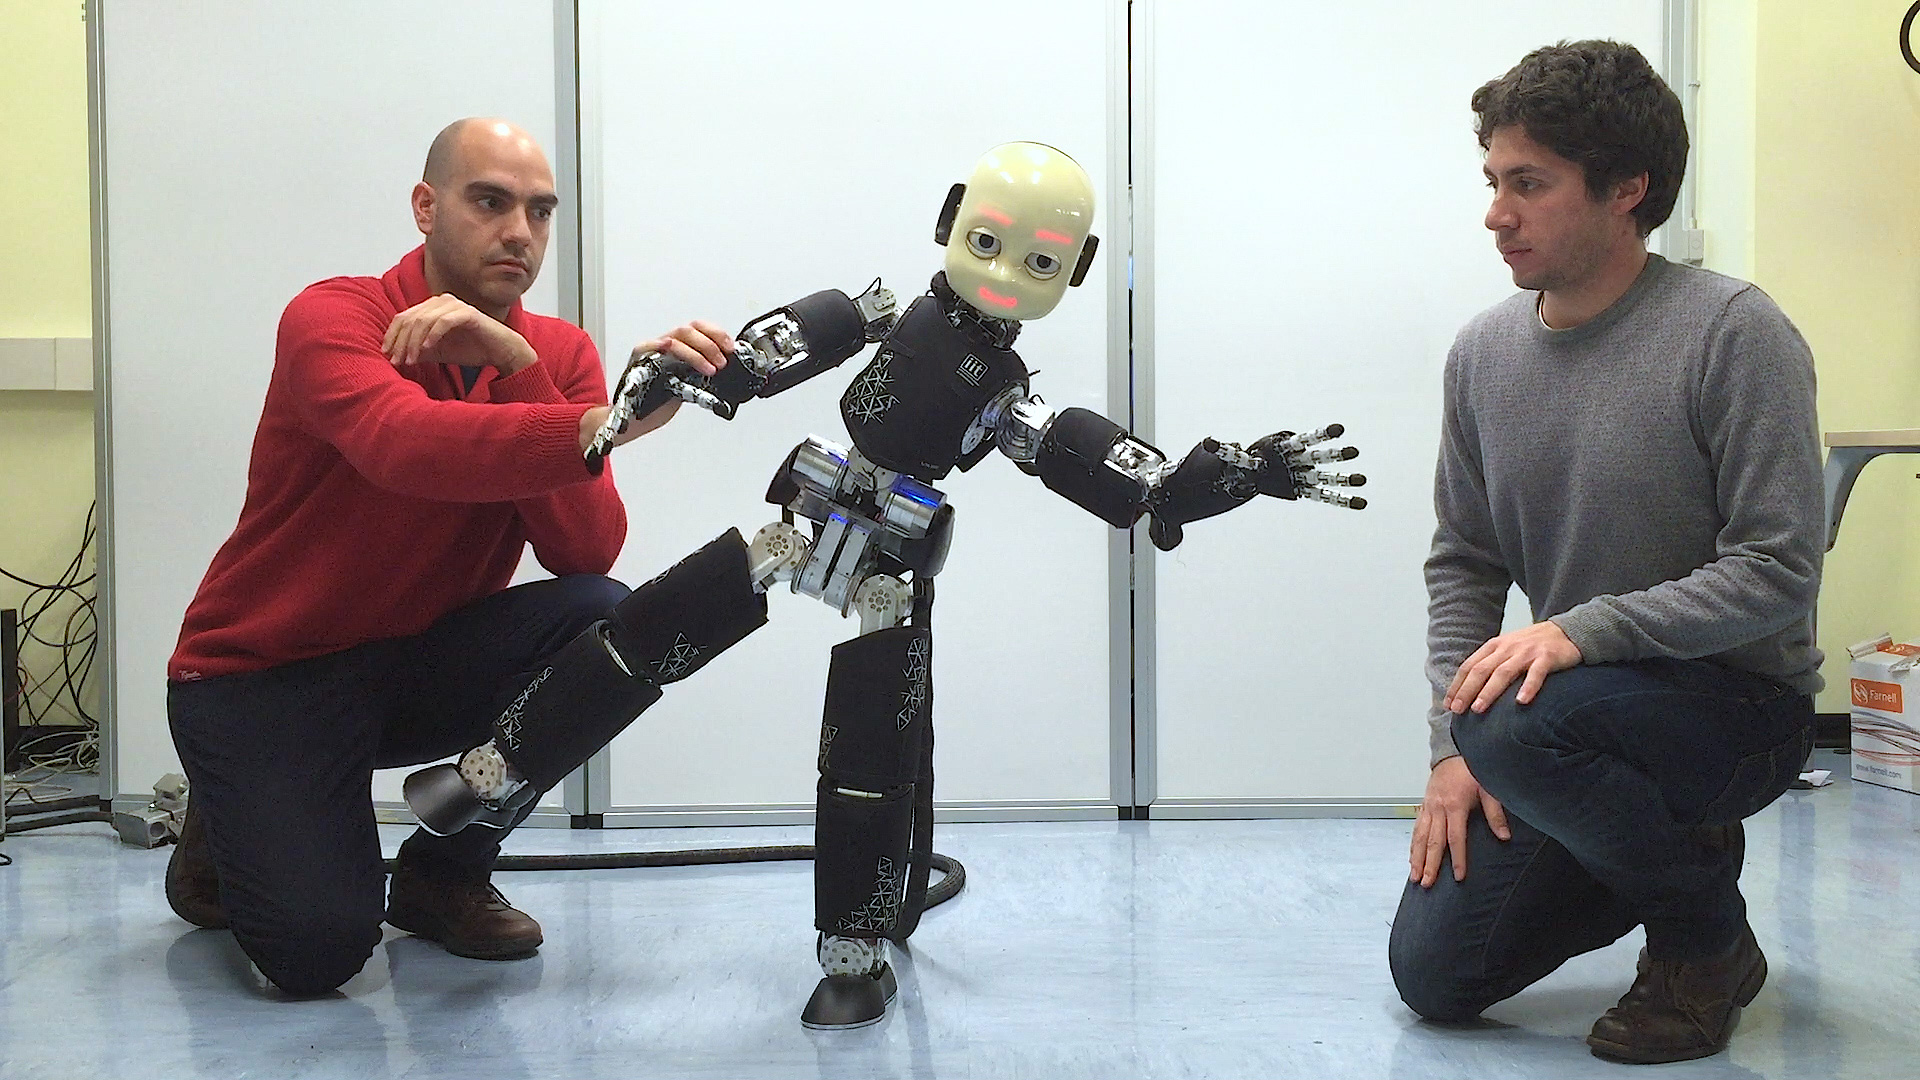
\includegraphics[width=0.65\columnwidth]{images/iCubInteractionOneFoot.jpg}
    \caption{A screen-shot of the one-foot balancing demo }
    \label{fig:oneFootBalnacing}
    }
\end{figure}

\begin{enumerate}
	\item Stabilization of the robot's momentum (expressed at the center-of-mass and with the inertial frame orientation), which is defined by
\begin{IEEEeqnarray}{RCL}
	\yesnumber
	H = \sum H_i = 
	\begin{pmatrix}
	m \dot{x} \\
	H_\omega
	\end{pmatrix},
	\nonumber
\end{IEEEeqnarray}
with $H_i$ the momentum of each link composing the multi-body system, $m$ the total mass of the robot, $x \in \mathbb{R}^3$ the position of the robot center-of-mass, and $H_\omega$ the angular momentum of the multi-body system. Let us recall that contrary to the case of a single rigid body, the possibility of expressing the angular momentum $H_\omega$ in terms of a proper angular velocity is still open. For this reason, we won't refer to a \emph{robot angular velocity} when stabilizing the humanoid angular momentum. 

The control of the robot momentum is achieved assuming the contact wrenches as a virtual control input in the dynamics of $H$. For instance, assuming that the robot is balancing on two feet, two external wrenches $f_L \in \mathbb{R}^6 $ and $f_R \in \mathbb{R}^6$ act on the left and right foot, respectively. Then, one has
\begin{IEEEeqnarray}{RCL}
	\label{centroidalMomentumDyn}
	\yesnumber
	\dot{H} = mg +^c X_L f_L +^c X_R f_R = mg + 
	\begin{pmatrix}
	^c X_L && ^c X_R 
	\end{pmatrix}	
	f,
\end{IEEEeqnarray}
where $^c X_L,^c X_R \in \mathbb{R}^{6\times6}$ are two proper projection matrices, and $f := (f_L^\top,f_R^\top)^\top$.
Since $f$ is assumed to be a control input, one can choose it so that $\dot{H} = \dot{H}^*$, where  $\dot{H}^*$ ensures that $x \rightarrow x_d$ and $H_\omega \rightarrow 0$. Clearly, at this level, one is left with a six-dimensional redundancy of the control input. This redundancy is exploited to minimize joint torques. 
	\item In the null space of the above task, we want the robot to assume a desired joint configuration, while having also some compliance. This is achieved by means of a postural task at the joint torque level, which exploits a proportional-derivative plus gravity compensation control strategy for stabilizing a desired joint reference.
\end{enumerate}

In the language of the \emph{Optimization Theory}, the above control objectives can be formulated as follows. 

\begin{IEEEeqnarray}{RCL}
	\IEEEyesnumber
	\label{optTorque}
	f^* &=& \argmin_{f}  |\tau^*(f)| \IEEEyessubnumber  \\
		   &s.t.& \nonumber \\
		   &&Cf < b \IEEEyessubnumber  \label{frictionCones} \\
		   && \dot{H}(f) = \dot{H}^* \IEEEyessubnumber \\
		   &&\tau^*(f) = \argmin_{\tau}  |\tau(f) - \tau_0(f)| 	\label{optPost} 
  \\
		   	&& \quad s.t.  \nonumber \\
		   	&& \quad \quad \ \dot{J}(q,\nu)\nu + J(q)\dot{\nu} = 0
		    \IEEEyessubnumber 	\label{constraintsRigid} \\
		   	&& \quad \quad \ \dot{\nu} = M^{-1}(S\tau+J^\top(q) f - h(q,\nu)) \IEEEyessubnumber \\
		   && \quad \quad \ 	\tau_0 = \bar{h}-\bar{J}^{\top}_j f- K_p (q_j-q^{des}_j)- K_d (\dot{q}_j-\dot{q}^{des}_j) \IEEEyessubnumber
		   \yesnumber
\end{IEEEeqnarray}
For the sake of completeness, in the above optimization problem one has
\begin{IEEEeqnarray}{RCL}
	\IEEEyesnumber 
	\dot{H}^* &=& 
	\begin{pmatrix}
		m(\ddot{x}_d - k_p(x-x_d)-k_d(\dot{x}-\dot{x}_d)) \\
		-k_\omega H_\omega -k_i \int_0^t  H_\omega ds
	\end{pmatrix}	 \IEEEyessubnumber\\
	\bar{h} &:=& h_j - M^\top_{bj}M^{-1}_b h_b \IEEEyessubnumber \\
	\bar{h} &:=& 
	\begin{pmatrix}
	h_b \\ h_j
	\end{pmatrix} =
	{C}(q, {\nu}) {\nu} + {G}(q), \quad h_b \in \mathbb{R}^6 \quad h_j \in \mathbb{R}^n
	 \IEEEyessubnumber \\
	\bar{J} &:=& J_j - J^{\top}_b M^{-1}_b M_{bj} \IEEEyessubnumber	\\
	M &=& 
	\begin{pmatrix}
		M_b && M_{bj} \\
		M^{\top}_{bj} && M_j
	\end{pmatrix}	 \quad M_b \in \mathbb{R}^{6\times 6}
	\quad M_{bj} \in \mathbb{R}^{6\times n}
	\quad M_b \in \mathbb{R}^{n\times n}\IEEEyessubnumber
\end{IEEEeqnarray}

Note that the additional constraint~\eqref{frictionCones} ensures that the desired contact wrenches $f$ belong to the associated friction cones. Once the optimum $f^*$ has been determined, the input torques $\tau$ are obtained by re-using the expression~\eqref{optPost}, i.e.
\begin{IEEEeqnarray}{RCL}
	\label{optTorqueFinal}
	\tau = \tau^*(f^*)
		   \yesnumber
\end{IEEEeqnarray}

Now, by direct calculations one can verify that the solution to the problem~\eqref{optPost} is an affine function versus the desired wrenches $f$, i.e. 
$\tau^* = A(q,\nu)f + b(q,\nu),$
where $A \in \mathbb{R}^{n\times 12}$ and $b \in \mathbb{R}^{n}$ two proper matrices. 
This leads to the following simplification of the optimization problem 
\begin{IEEEeqnarray}{RCL}
	\label{optTorque2}
	\IEEEyesnumber
	f^* &=& \argmin_{f}  |\tau^*(f)|  \IEEEyessubnumber \\
		   &s.t.& \nonumber \\
		   &&Cf < b \IEEEyessubnumber  \label{frictionCones2} \\
		   && \dot{H}(f) = \dot{H}^* \IEEEyessubnumber \\
		   &&\tau^*(f) = A(q,\nu)f + b(q,\nu) \IEEEyessubnumber
		   \yesnumber
\end{IEEEeqnarray}
The above control algorithm has run at both review meetings of the CoDyCo project.

\section{Modelling and control design for a humanoid balancing on a thin carpet} 
\label{sec:modellingAndControlSoft}
This section discusses the modification of the control algorithm~\eqref{optTorque} for dealing with compliant  contacts.
 Prior to the control design, however, we present a simple model for the carpet.

\subsection{Modelling}
To introduce the reader to the model of a compliant carpet, we first consider the planar case, and then address the three-dimensional case.

\subsubsection{A case study: the planar case}

Figure~\ref{fig:compliantCarpet} shows a uniform force distribution acting on a compliant carpet of height~$h$. The resultant force due to the distribution is denoted by $F$. The force distribution induces a compression of the compliant carpet and, assuming uniform carpet characteristics, the  compression is equally distributed. So,  the carpet is horizontal even after the compression due to the force distribution. Now, assume that the mapping $F: z_M \rightarrow F_E$ is known -- or properly estimated --  in the case shown in Figure~\ref{fig:compliantCarpet}. The following details how to evaluate the resultant force and torque acting from the carpet to the contact surface  when it is not uniformly compressed. To this purpose, we make the following assumptions.

 \begin{figure}[t]
     \centering{
     % \includsvg{imgs/model}
         \def\svgwidth{0.7\columnwidth}         
         \input{images/softFloor.eps_tex}
     \caption{A compliant carpet subject to a uniform force distribution}
     \label{fig:compliantCarpet}
   }
\end{figure}



\begin{assumption}
\label{hp:uniformity} 
Throughout the paper, we assume the following.
\begin{enumerate}
    \item The carpet characteristics are isotropic.
    \item The soft carpet can be approximated as a continuum of springs. In addition, each infinitesimal spring can  exert only a vertical force.
    \item An off-line estimation procedure provides us with the mapping $F = F_E(z_M)$ when a uniform force distribution $f(\cdot)$ is applied to the carpet.
\end{enumerate}
\end{assumption}

Let $l$ denote the length of the compliant carpet subject to the uniform force distribution. As a consequence of assumptions~\ref{hp:uniformity}.1 and~\ref{hp:uniformity}.3, one has:

\begin{equation}
\label{forceFromIntegral}
F_E(z_M) = \int_{a}^{b} f(z_M) dx = f(z_M) l.
\end{equation}
So, we can evaluate the force distribution $f(z)$ from the estimated force $F_E(z_M)$, 

\begin{equation}
f(z) = \frac{F_E(z)}{l}.
\end{equation}

Then, 
Eq.~\eqref{forceFromIntegral} can be used to evaluate  the total force applied from the carpet to a generic contact surface, i.e.

\begin{equation}
\label{forceFromIntegral1}
F = \int_{a}^{b} f(z(x)) dx,
\end{equation}
with $z(x)$  a proper function describing the shape of the  contact surface on a domain $x~\in~[a,b]$.
%, so that $l_n = b-a$. 
Also, in view of the assumption~\ref{hp:uniformity}.2, the torque about a point located at $x = \bar{x}$ of the carpet can  be easily computed as:
\begin{equation}
\label{momentFromIntegral}
M = \int_{a}^{b} f(z(x))(x-\bar{x}) dx.
\end{equation}

\subsubsection{The case of a flat contact surface and a linear force distribution}

Assume that the flat surface in Figure~\ref{fig:compliantCarpet} bends as shown in 
Figure~\ref{fig:compliantCarpetBent}. Then, its shape can be characterized by a line of slope $\tan(\theta)$, i.e

\begin{equation}
\label{surfaceBent}
z(x) = z_M + \tan(\theta) (x-x_M),
\end{equation}
with $(x_M,z_M)$ the coordinates of the central point of the flat plate.
In addition,
assume  also that the estimated force $F = F_E(z_M)$ is linear with respect to the carpet's compression, i.e.
\begin{equation*}
    F_E(z_M) = K(h-z_M),
\end{equation*}
which implies 
\begin{equation}
    \label{forceDistributionLinear}
    f(z) = k(h-z),
\end{equation}
with $k:= K/l$. Then, the total force and torque exerted from the compliant carpet to the flat surface is given by  \eqref{forceFromIntegral1} and~\eqref{momentFromIntegral} evaluated with~\eqref{forceDistributionLinear} and~\eqref{surfaceBent}, i.e.

\begin{subequations}
    \begin{alignat}{2}
        F &= \int_{x_M-\frac{l}{2}\cos(\theta)}^{x_M+\frac{l}{2}\cos(\theta)} f(z(x))dx=kl\cos(\theta)\left(h-z_M \right) \\\nonumber
        M &=\int_{x_M-\frac{l}{2}\cos(\theta)}^{z_M+\frac{l}{2}\cos(\theta)} f(z(x))(x{-}\bar{x}) dx \\ 
          &= kl\cos(\theta) \left[ (h-z_M)\left(x_M-\bar{x} \right) - 
          \frac{l^2}{12} \sin(\theta)\cos(\theta) \right] 
    \end{alignat}
\end{subequations}
%
\begin{figure}[t]
    \centering{
    % \includsvg{imgs/model}
        \def\svgwidth{0.7\columnwidth}         
        \input{images/softFloorBent2D.eps_tex}
    \caption{A compliant carpet subject to a non-uniform force distribution}
    \label{fig:compliantCarpetBent}
    }
\end{figure}

The process of finding the solutions to the above integral is simplified by applying the variable transformation $\xi = x - x_M$, which renders the limits of integration equal to $-0.5l \cos(\theta)$ and $0.5l \cos(\theta)$. This hint is used for calculating the integrals in the more-complex 3-D case.

Note that if the torque $M$ is expressed with respect to the central point $(x_M,z_M)$ of the plate, one has:
\begin{subequations}
    \begin{alignat}{2}
        F &=kl\cos(\theta)\left(h-z_M \right) \\
        M &= -k
          \frac{l^3}{12} \sin(\theta)\cos^2(\theta) 
    \end{alignat}
\end{subequations}

As shown in Figure~\ref{fig:compliantCarpetBent},
positive angles $\theta$ produce negative torques, 

\subsubsection{The three-dimensional case}
Analogously to the planar case, this section addresses the modeling of the forces and torques applied from a compliant carpet to a contact surface by considering the three-dimensional case. To this purpose, we still assume that Assumption~\ref{hp:uniformity} holds, modulo straightforward modifications for handling the three-dimensional case. In particular, we assume that an estimation procedure is performed when the contact surface is a flat, rectangular plate of length $l$ and width $d$ -- see Figure~\ref{fig:compliantCarpet3D}. In addition, we also assume that the estimation procedure consists of applying  a uniform force distribution  so that  the flat plate compresses the carpet uniformly. Hence, the estimated force takes the following form:

\begin{equation}
\label{eq:forcesDist3DEst}
F_E(z) = e_3 \int_{x_0}^{x_1} \int_{y_0}^{y_1} f(z) dx dy = f(z) l d e_3,
\end{equation}
with 
%$e_3 = (0 \quad 0 \quad 1)^\top$,  and 
$f(z)$  the vertical force distribution per surface. Hence, the force distribution can be evaluated as follows:
\begin{equation}
\label{fromForceToDistr3D}
f(z) = \frac{|F_E(z)|}{ld}.
\end{equation}
In light of the above, the force and torque due to a generic contact surface is given by:
\begin{subequations}
\label{forceTorque3DGeneral}
    \begin{alignat}{2}
\label{eq:forcesDist3DE}
F &= e_3 \int\int_{{D}} f(z) dx dy, \\
\label{eq:torqueDist3DE}
M &= 
% \int \int S(p-p_0) e_3 f(z) dx dy =
\int \int_{{D}}
%\begin{pmatrix}
%    y - \bar{y} \\
%    \bar{x} - x \\
%    0
%\end{pmatrix}
f(z)S(p-\bar{p})e_3 dx dy, 
    \end{alignat}
\end{subequations}
with $p=(x \quad y \quad z)^\top$ a point of the contact surface,  
$\bar{p} = (\bar{x} \quad \bar{y} \quad \bar{z})^\top$ the point w.r.t. which the torque is expressed, and $D \subset \mathbb{R}^2$ a proper integration domain associated with the contact surface configuration.
% , and $S(\cdot) \in \mathbb{R}^3$ the skew-symmetric matrix associated with the cross product operator in $\mathbb{R}^3$, i.e. $u \times v = S(u)v$.
\begin{figure}[t]
    \centering{
    % \includsvg{imgs/model}
        \def\svgwidth{0.75\columnwidth}         
        \input{images/softFloor3DBent.eps_tex}
    \caption{A compliant carpet subject to a non-uniform force distribution}
    \label{fig:compliantCarpet3D}
    }
\end{figure}
%
%\begin{figure}[t]
%    \centering{
%    % \includsvg{imgs/model}
%        \def\svgwidth{0.75\columnwidth}         
%        \input{figures/softFloor3D.eps_tex}
%    \caption{A compliant floor subject to a non-uniform force distribution}
%    \label{fig:compliantCarpet3D}
%    }
%\end{figure}

\subsubsection{The case of a flat contact surface and a linear force distribution}
\label{compliantCarpet3D}
Assume that the contact surface is flat -- see Figure~\ref{fig:compliantCarpet3D} -- so it can be characterized by the following equation

\begin{equation}
\label{distributionPlane}
n^\top p = 0,
\end{equation} 
with $n \in \mathbb{R}^3$ the unit vector perpendicular to the  surface.

\begin{boldLemma}
\label{lemma3D}
Assume that Assumption~\ref{hp:uniformity} holds, and that the force distribution $f(\cdot)$ associated with the compliant carpet  is linear with respect to the height, i.e.
\begin{equation}
\label{distributionLinear3D}
f(z) = k(h-z).
\end{equation}
Let a flat, rectangular surface, of length $l$ and width $d$, be in full-contact with the compliant carpet. Then, the force-torque acting on the  rectangular surface at the equilibrium configuration is given by: 
\begin{subequations}
\label{forceTorqueOn3DBentPlate}
    \begin{alignat}{2}
\label{force3D}
F &= kld|n^\top e_3|\left(h-z_M \right)e_3 \\
\label{torque3D}
M &= S(p_M - \bar{p})F + \frac{kld}{12}|n^\top e_3|S(e_3)\Lambda(\imath,\jmath)e_3 
    \end{alignat}
\end{subequations}
with 
\begin{equation}
\Lambda = d^2 \jmath \jmath^\top + l^2 \imath \imath^\top ,
\end{equation}
 $p_M$  the central point of the rectangular surface,  
%$\bar{p}~{=}~(\bar{x},\bar{y},\bar{z})$ the point with respect to which the torque $M$ is expressed, 
and $\imath$ and 
$\jmath$ two unit, perpendicular vectors parallel to the rectangle's borders associated with the length and the width, respectively.
\end{boldLemma}

The proof is given in the Appendix. The above Lemma points out that the total force $F$ depends on the normal $n$ to the plane representing the flat plate, but it does not depend on the angle about this normal (i.e. the \emph{yaw} angle about the normal $n$). Clearly, the force $F$ also depends on how much the  plate immerses into the soft carpet, and this dependence comes from the term $(h-z_M)$ in Eq.~\eqref{force3D}. The expression of the torque $M$, instead, is the sum of two terms: the torque due to the force $F$ applied at the point  $\bar{p}$ plus a term  depending only on the relative orientation of the plate w.r.t. the inertial frame. Note that if the plate is parallel to the plane $x-y$ of the inertial frame, then $\imath^\top e_3 = 0$ and 
$\jmath^\top e_3 = 0$. As a consequence, the second term on the right hand side of~\eqref{forceTorqueOn3DBentPlate} is equal to zero, and so is the momentum $M$ when expressed with respect to $p_M$ (i.e. $\bar{p}=p_M$). 

\subsubsection{Constraints associated with the flat plate due to friction}
Consider Figure~\ref{fig:compliantCarpet3D}, where $v \in \mathbb{R}^3$ denotes the velocity of the point $p_M$, and $\omega \in \mathbb{R}^3$ the angular velocity of the flat plate, both expressed with respect to the inertial frame. Then, it is reasonable to assume that friction effects  forbid any rotation of the plate about the axis $n$ as long as friction forces belong to the associated friction cones, i.e. $n^\top \omega = 0$. In addition, it is also reasonable  to assume that friction effects forbid the velocity of any point of the plate to be tangential to the plate itself. It is straightforward to verify that the velocity of any point $p$ of the flat plate has null tangential velocity if and only if the velocity of the point $p_M$ has  null tangential velocity when $n^\top \omega = 0$. In light of the above,  we assume that as long as friction forces belong to the associated friction cones, one has:
\begin{subequations}
\label{constraintsWithVerticalMotion}
    \begin{alignat}{3}
\imath^\top v &= 0 \\
\jmath^\top v &= 0 \\
n^\top \omega &= 0 
    \end{alignat}
\end{subequations}
The above equations point out that the flat plate can rotate only about the axes $\imath$ and $\jmath$, and can also go "up-and-down" due to the compliance of the carpet. When coming to practice, however, it is also reasonable to assume that the vertical speed of the point $p_M$ is equal to zero, i.e.
\begin{equation}
\label{constraintsNoVerticalMotion}
e^\top_3 v = 0
\end{equation}
Let us justify this additional hypothesis.
Eq.~\eqref{force3D} shows that the vertical force at the equilibrium configuration exerted from the carpet to the plate is given by
\begin{equation}
F_z = kld|n^\top e_3|\left(h-z_M \right). \nonumber
\end{equation}
Now, without loss of generality, assume that the point $p_M$ is the plate's center of mass. Then, the force balance along the $z$ axis writes:
\begin{equation}
m_p\ddot{z}_M = 
%F^{Ext}_z 
-k_v \dot{z}_M + kld|n^\top e_3|\left(h-z_M \right) -m_pg  \nonumber
\end{equation}
where $m_p$ is the mass of the plate, and $k_v$ the viscous coefficient associated with the compliant carpet. In particular, thin compliant carpet are
typically  associated with very high value of $k_v$, which implies fast convergence of the plate vertical velocity to zero, i.e. $\dot{z}_M \rightarrow 0$. Also,  from the above equation, it is clear that at the equilibrium configurations with a flat plate almost parallel to the ground, i.e. $|n^\top e_3| \approx 1$, one has 
\begin{equation}
 z_M  \approx h-\frac{m_pg}{kld}  . \nonumber
\end{equation}
Since the weight of the plate is constant, then the height $z_M$ converges to the same value independently of an external, vanishing perturbation applied to the plate. This fact combined with the high value of carpet's damping justify the assumption~\eqref{constraintsNoVerticalMotion}.



\subsubsection{Kinematic constraints and contact forces associated with the robot's feet}


Assume that the robot is balancing on both feet, underneath which there is the compliant carpet characterized by the equations presented above. In view of Eq.~\eqref{constraintsWithVerticalMotion}-\eqref{constraintsNoVerticalMotion}, the constraints acting on both feet  can be compactly written as:
\begin{IEEEeqnarray}{RCL}
\label{constraintsWithVerticalMotionCompact}
 \IEEEyesnumber
 \bar{H} ^{\mathcal{I}} {v}_f &=& 0, 
\end{IEEEeqnarray}
with 
\begin{IEEEeqnarray}{RCL}
	\IEEEyesnumber
	\bar{H} &=& 
	\begin{pmatrix}
		{H}(\imath_L,\jmath_L,n_L) && 0_{4\times 6} \\
 		0_{4\times 6} && {H}(\imath_R,\jmath_R,n_R)
	\end{pmatrix} \IEEEyessubnumber  \\
	\label{feetvelocity}
 v_f &=& 
 \begin{pmatrix}
\bm{v}_L \\
 \bm{v}_R
\end{pmatrix}, \IEEEyessubnumber
\end{IEEEeqnarray}
and $(\imath_L,\jmath_L,n_L)$ and $(\imath_R,\jmath_R,n_R)$ two frames attached to the left and right foot, respectively (as indicated in Figure~\eqref{fig:compliantCarpet3D}b and  $\bm{v}_L$ and $\bm{v}_R$ the linear and angular velocity of the central point of the robot's feet, respectively. Now, the feet velocity $ ^{\mathcal{I}}{v}_f$ can be expressed in terms of the robot velocity $\nu$ though its Jacobian, i.e. 
\[ ^{\mathcal{I}}{v}_f = J(q)\nu.\]
By substituting the above equation into~\eqref{constraintsWithVerticalMotionCompact}, one obtains
\begin{IEEEeqnarray}{RCL}
\label{constraintsCompactComplJBar}
 \IEEEyesnumber
 {J}_s(q)\nu &=& 0\IEEEyessubnumber \\
 {\dot{J}}_s(q)\nu + {J}_s(q)\dot{\nu} &=& 0\IEEEyessubnumber
 \label{constraintsCompactComplJBar}
\end{IEEEeqnarray}
where
\begin{IEEEeqnarray}{RCL}
\label{constraintsCompactJBar}
 \IEEEyesnumber
 {J}_s(q) &:=& \bar{H}(q)J(q). 
\end{IEEEeqnarray}
Hence, the constraint equations when the robot stands on a compliant carpet have the same form of  those when standing on rigid constraints (compare Eqs.~\eqref{constraintsCompactComplJBar} and~\eqref{constraintsRigid}). What does change between these two situations is the number of rigid constraints acting on the system. In fact, in the case the robot stands on rigid contacts, one has 12 kinematic constraints, while when the humanoid balances on the soft carpet, %described in  Section~\ref{sec:modelCarpet}, 
one has 8 rigid constraints acting on the system. 

The rigid constraints generate eight contact \emph{forces} $f^{rigid} \in \mathbb{R}^8$, which must be taken into account in the dynamic equation, i.e.
\begin{IEEEeqnarray}{RCL}
    \label{eq:system_dynamicsCarpet}
       {M}(q)\dot{{\nu}} + {C}(q, {\nu}) {\nu} + {G}(q) &=&  B \tau 
       + {J}_s^\top(q) f^{rigid} + J^\top(q) f^{comp} 
\end{IEEEeqnarray}
By combining the above equation with the constraints~\eqref{constraintsCompactComplJBar}, one can find an expression of the contact forces $f^{rigid}$, which thus depend on the  torque $\tau$, and can be assumed as an artificial control input. Note that the effect of the compliant forces $f^{comp}$ in Eq.~\eqref{eq:system_dynamicsCarpet} is also taken into account. Let $f^{comp}_{L} \in \mathbb{R}^6$ and $f^{comp}_{R}\in \mathbb{R}^6$ denote the compliant wrenches acting on the left and right foot, respectively. Assuming that the contact torques $M$ in  Eq.~\eqref{forceTorqueOn3DBentPlate} are expressed w.r.t. the feet central point, i.e. $ \bar{p} = p_M $, and that the feet can be approximated as two rectangles of the same dimension, one has
\begin{IEEEeqnarray}{RCL}
\label{fcompl}
f_{comp} =
\begin{pmatrix}
f^{comp}_{L}  \\
f^{comp}_{R} 
\end{pmatrix}=kld
\begin{pmatrix}
|n_L^\top e_3|\left(h-z^{L}_M \right)e_3  \\
 \frac{1}{12}|n_L^\top e_3|S(e_3)\Lambda(\imath_L,\jmath_L)e_3 \\
|n_R^\top e_3|\left(h-z^{R}_M \right)e_3  \\
  \frac{1}{12}|n_R^\top e_3|S(e_3)\Lambda(\imath_R,\jmath_R)e_3, 
\end{pmatrix}
\end{IEEEeqnarray}
with $z^{L}_M$ and $z^{R}_M$ the third components of the position vectors $p^{L}_M$ and $p^{R}_M$ describing the central points of the feet, i.e. 
$z^{L}_M = e^\top_3 p^{L}_M$ and $z^{R}_M = e^\top_3 p^{R}_M$.

\subsection{Control design}

Recall that the control objective is the asymptotic stabilization of the robot momentum, the rate of change of which equals the net external wrench acting on the system. In the case the robot is balancing on the compliant carpet described in Section~\eqref{compliantCarpet3D}, one then has
\begin{IEEEeqnarray}{RCL}
	\label{centroidalMomentumDynComp}
	\yesnumber
	\dot{H}(f^{rigid}) =  mg + 
	\begin{pmatrix}
	^c X_L, && ^c X_R 
	\end{pmatrix}	
	(\bar{H}^\top(q) f^{rigid} + f^{comp}),
\end{IEEEeqnarray}
where $f^{rigid}$, being dependent on the input torques $\tau$, can be assumed as a control input in the above dynamics. 

In light of the above, the control problem~\eqref{optTorque} is formulated as follows.

\begin{IEEEeqnarray}{RCL}
	\IEEEyesnumber
	\label{optTorqueCompliant}
	f^{rigid}_* &=& \argmin_{f^{rigid}}  |\tau^*(f^{rigid})| \IEEEyessubnumber  \\
		   &s.t.& \nonumber \\
		   &&Cf^{rigid} < b \IEEEyessubnumber  \label{frictionConesCompliant} \\
		   && \dot{H}(f^{rigid}) = \dot{H}^* \IEEEyessubnumber \\
		   &&\tau^*(f^{rigid}) = \argmin_{\tau}  |\tau(f^{rigid}) - \tau_0(f^{rigid})| 	\label{optPostCompliant} 
  \\
		   	&& \quad s.t.  \nonumber \\
		   	&& \quad \quad \ \dot{J}_s(q,\nu)\nu + J_s(q)\dot{\nu} = 0
		    \IEEEyessubnumber 	\label{constraintsRigidCompliant} \\
		   	&& \quad \quad \ \dot{\nu} = M^{-1}(S\tau+{J}_s^\top(q) f^{rigid} + J^\top(q) f^{comp}  - h(q,\nu)) \IEEEyessubnumber \\
		   && \quad \quad \ 	\tau_0 = \bar{h}{-}\bar{J}^{\top}_j(\bar{H}^\top(q) f^{rigid} + f^{comp}){-} K_p (q_j-q^{des}_j){-} K_d (\dot{q}_j-\dot{q}^{des}_j) \IEEEyessubnumber
		   \yesnumber
\end{IEEEeqnarray}

Analogously to what we discussed in Section~\ref{sec:firstSecondValid}, the above control problem is equivalent to:
\begin{IEEEeqnarray}{RCL}
	\label{optTorqueSoft}
	\IEEEyesnumber
	f^{rigid}_* &=& \argmin_{f^{rigid}}  |\tau^*(f^{rigid})|  \IEEEyessubnumber \\
		   &s.t.& \nonumber \\
		   &&Cf^{rigid}< b \IEEEyessubnumber  \label{frictionCones3} \\
		   && \dot{H}(f) = \dot{H}^* \IEEEyessubnumber \\
		   &&\tau^*(f) = A(q,\nu)(\bar{H}^\top(q) f^{rigid} + f^{comp}) + b(q,\nu)  \label{optTorqueOne}  \IEEEyessubnumber
		   \yesnumber
\end{IEEEeqnarray}
and once the optimal solution  $f^{rigid}_*$ is determined, we apply again Eq.~\eqref{optTorqueOne} to determine the input torques to the robot. 

The above control algorithm will be implemented for the third year demo review meeting when the humanoid must balance on two feet and on a compliant carpet.

\newpage

\section{Control design for  humanoids balancing on seesaws} 
\label{sec:controllerSeeSaw}

\subsection{The equation of motion of the seesaw} 
\label{sec:eqmotion}
\begin{figure}[t]
    \centering{
    % \includsvg{imgs/model}
        \def\svgwidth{1\columnwidth}         
        \input{images/seesaw.eps_tex}
    \caption{The semi-cylindrical seesaw}
    \label{fig:seesaw}
    }
\end{figure}

The equation of motion of the seesaw are derived by considering it as a rigid body subject to the rolling constraint. Let $m_s$ and $I_s$ denote the mass and the inertia matrix of the seesaw, and $^{\mathcal{I}} v_s$ and $^{\mathcal{I}} \omega_s$ the linear velocity of its center of mass and its angular velocity, respectively. Then,  the momentum of the seesaw $H_s \in \mathbb{R}^6$ is defined by
\begin{IEEEeqnarray}{RCL}
 \IEEEyesnumber
    H_s :=
 	\begin{pmatrix}
 	m_s \ ^{\mathcal{I}} v_s \\
 	I_s \ ^{\mathcal{I}} \omega_s
 	\end{pmatrix},
\end{IEEEeqnarray}
and the equation of motion= are given by
\begin{IEEEeqnarray}{RCL}
 \IEEEyesnumber
    \dot{H}_s &=& 
 	\sum_i w_{ext_i}   
\end{IEEEeqnarray}
subject to the following constraints 
\begin{IEEEeqnarray}{RCL}
 \IEEEyesnumber
 	\label{constraintsSeesaw}
 	^{\mathcal{I}} v_p &=&0.\IEEEyessubnumber \label{rollingConstraint} \\
 	 ^{\mathcal{I}} \omega_s{^\top}  e_2 &=& 0  \IEEEyessubnumber \\
 ^{\mathcal{I}} \omega_s{^\top}  e_3 &=& 0  \IEEEyessubnumber
\end{IEEEeqnarray}
with $w_{ext}$ the external wrenches applied to the seesaw. The kinematic constraints~\eqref{constraintsSeesaw} express the following facts: 
\begin{itemize}
\item The seesaw cannot rotate about the axes $e_2$ and $e_3$ of the inertial frame.
\item The contact point between the seesaw and the floor possesses null velocity. This, along with the constraints on the seesaw angular velocity,  ensures that all points of the contact line between the  seesaw and the floor have zero velocity.
\end{itemize}
The satisfaction of the above constraints is ensured as long as the contact wrench $w_c$ (see Figure~\ref{fig:seesaw} ) belong to the associated friction cones.

\section{Estimation algorithms} 
\label{sec:estimation}

\subsection{Estimation of the floating base} 
\label{sec:estimationFloatingBase}

\subsection{Estimation of the floor compliance} 
\label{sec:estimationFloorCompliance}

\bibliographystyle{apalike}
\bibliography{D5.3}

\end{document}

%%% Local Variables:
%%% mode: latex
%%% TeX-master: t
%%% save-place: t
%%% End:
